\documentclass[12pt,a4	]{report}
\usepackage[frenchb]{babel}

\usepackage[usenames,dvipsnames]{color}
\usepackage[utf8]{inputenc}
\usepackage{textcomp}
\usepackage[T1]{fontenc}
\usepackage{lmodern}	
\usepackage{bibunits}
\usepackage{graphicx}
\usepackage{wrapfig}
\usepackage{glossaries}
\makeglossaries
\usepackage{float}
\usepackage{cite}
\usepackage{caption}
\usepackage{amsmath,mathtools}
\usepackage{subcaption}

\newacronym{w3c}{W3C}{World Wide Web Consortium}
\newacronym{rdf}{RDF}{Resource Description Framework}
\newacronym{strdf}{stRDF}{spatial and temporal Resource Description Framework}
\newacronym{lod}{LOD}{Linked Open Data, Web de données}
\newacronym{sparql}{SPARQL}{Protocol and RDF Query Language}
\newacronym{stsparql}{stSPARQL}{spatial and temporal Protocol and RDF Query Language}
\newacronym{uri}{URI}{Uniform Resource Identifier}
\newacronym{iri}{IRI}{Internationalized Resource Identifier }
\newacronym{sql}{SQL}{Structured Query Language}


\begin{document}


\section*{État de l'art}
\subsubsection*{Introduction}
\paragraph{}
Dans ce chapitre nous introduisons les différentes technologies qu'on va utiliser dans notre étude ainsi que les travaux de recherche liée à cette problématique; toute en essayant d'analyser les différentes approches. Afin de mettre en place la solution que nous avons proposé.  Nous aborderons ce dernier point dans le prochain chapitre.

\subsection*{Apperçu du domaine}
\paragraph{}
Notre étude a la particularité d’englober le domaine de la fouille de données et du Web sémantique. 
En effet, on utilise les techniques de la fouille pour l'extraction des données depuis les différentes sources d'informations, et le Web sémantique afin de donner au métadonnées une structure plus lisible par la machine.
\subparagraph{}
Dans ce chapitre on présente les téchnologies du Web sémantique que nous avons utilisé, puis nous effectuons une étude préliminère autour des travaux de recherche qui précède notre étude toute en introduisant les concepts et la problèmatique de notre sujet.
\subsection*{Technologies du Web sémantique}
\subsubsection*{Intérêt du Web sémantique}
\paragraph{}
Le Web sémantique est un domaine de recherche né des travaux de Tim Berners-Lee l'un des pionniers dans ce secteur~\cite{Berners-lee2001} dont le but était d'ajouter du sens aux contenus du Web. Ce n'est pas une question d'ajouter une autre alternative du Web mais c'est plustôt d'étendre le Web actuel dans le but d'utiliser et manipuler le maximum de son contenu informatiquement. En clair, c'est de permettre à des programmes informatiques de traiter un ensemble étendu de données issues du Web.
\subsubsection*{Modèle RDF}
\paragraph{}
Au centre du Web sémantique, comme la brique d’argile qui permet d’ériger les plus grands édifices, se trouve le modèle \gls{rdf} . RDF\footnote{http://www.w3.org/RDF/} est un standard de \gls{w3c}, il se base sur un modèle de graphe sous forme de triplets (sujet, prédicat, objet) qui permettent d'exprimer tous types d'assertions. Il s’agit d’un cadre de description de ressources, d’une façon formelle sur le Web.
C’est la première brique de standard du Web sémantique qui recouvre à la fois un modèle et plusieurs syntaxe pour publier des données variées sur le Web.
\subparagraph{}
Dans RDF ~:
\newline
\begin{itemize}
\item Les ressources sont un concept de base du Web sémantique, tout ce qui peut être référencé est une ressource. Dans un contexte plus technique~: on déduit que tout ce qui peut être identifié par un \gls{uri} / \gls{iri} peut être considéré comme ressource.
\item Un ensemble d’attributs décrivent la ressource, qui possèdent des caractéristiques et des relations avec d’autres ressources.
\item Le cadre standardise la syntaxe de ces descriptions, les modèles et les langages.
\end{itemize}
\subparagraph{}
La plus petite structure de description en RDF est le triplet.
\begin{figure}[H]
\centering
\centering
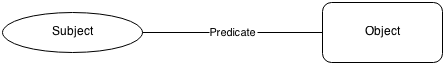
\includegraphics[width=8cm]{tripletrdf.png}
\caption{triplet RDF}

\end{figure}
\subparagraph{}
Un triplet décrit une ressource, l’associe à une propriété et une valeur de cette propriété qui peut être une nouvelle ressource liée.
\newline
Par exemple “Moncef a écrit une page QuadsRDF.html à propos des quadruplets RDF” peut être décomposée en deux triplets ayant comme sujet “QuadsRDF.html”: <QuadsRDF.html, auteur, Moncef> et <QuadsRDF.html, thème, quadruplets RDF>.
\newline
On peut schématiser cela de la manière suivante:
\begin{figure}[H]
\centering
\centering
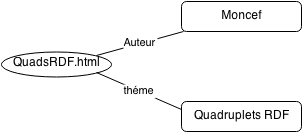
\includegraphics[width=8cm]{Diag.png}
\caption{Deux Triplets liés au même sujet}

\end{figure}
\subsubsection*{SPARQL}
\paragraph{}
Si RDF fournit un modèle universel de représentation de métadonnées. D'autres niveaux de traitements ont été standariser au dessus de lui et notament l'interrogation de ces métadonnées.
\gls{sparql} fournit le langage d'interrogation du Web sémantique, et en cela il est à RDF ce que \gls{sql} est au bases de données relationnelles.
\subparagraph{}
SPARQL est un langage d'interrogation de graphe RDF dont l'énoncé de base est lui aussi un triplet (ressource, propriété, valeur).Il est une recommandation du W3C depuis juillet 2008.
Poser une question en SPARQL consiste à écrire un graphe requête pour lequel on cherche des occurences dans le graphe cible.
\subsubsection*{N-Quads}
\paragraph{}
N-Triples est une simple syntaxe ligne délimitée( line-delimited) pour les graphes RDF. N-Quads\footnote{http://sw.deri.org/2008/07/n-quads/}, un format qui s'étend N-Triples avec le contexte. Chaque triplet dans un document N-Quads peut avoir une valeur de contexte en option:
\newline
<subjet> <prédicat> <objet> <contexte>.
\subparagraph{}
La notion de provenance est essentiel lors de l'intégration des données provenant de différentes sources ou sur le Web . Par conséquent, l'état de l'art des référentiels RDF (sujet, prédicat, objet, contexte) quadruplet, lorsque le contexte indique généralement la provenance d'une déclaration donnée.
\newpage
\subsection*{Base de Connaissances}
\subsubsection*{Introduction}
\paragraph{}
Une base de connaissance regroupe des informations spécifiques à un domaine donné, sous un format exploitable par un ordinateur. Elle peut contenir des régles, des faits ou d'autres représentations. Les base de connaissances regroupent des informations structurées et nous particulièrement on cherche à exploiter ces informations pour les mettres dans une nouvelle structure plus facilement exploitable par la machine.

\subsubsection*{DBpedia}
\paragraph{}

C'est un projet universitaire et communautaire d’extraction et d’exploitation automatique des données de wikipedia. C’est également un ensemble de données structurées et normalisées au format du Web sémantique.
\begin{wrapfigure}{r}{0.7\textwidth}
\vspace{-10pt}
\begin{center}
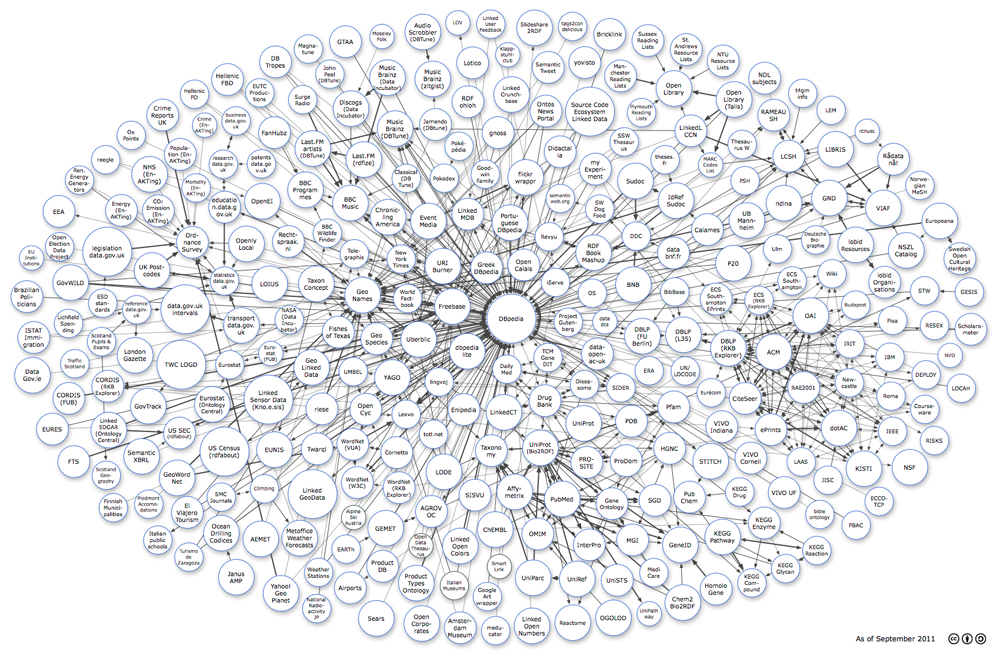
\includegraphics[width=0.50\textwidth]{dbpedia.png}
\end{center}
\vspace{-15pt}
\caption{DBpedia}
\vspace{-10pt}
\end{wrapfigure}
DBpedia 3.9 est la dernière version de DBpedia datant de Juin 2013.
\subparagraph{}
Cette base de connaissance est écrite en Scala et Java. Elle adopte les normes du Web sémantique et du réseau Linked Open Data. Pour chaque document encyclopédique, il existe une page de ressources contenant toutes les données sous forme de triplets RDF.
\newpage
\subsubsection*{YAGO}
YAGO\footnote{http://www.mpi-inf.mpg.de/yago-naga/yago/} est une large base de connaissance sémantique, délivré de Wikipedia, WordNet et GeoNames. Actuellement elle contient plus de 10 million entités (personnes, organisations, villes, etc..) et plus de 120 million faits de ces entités.
\newline
Les caractéristiques principales de YAGO :
\begin{itemize}
\item Une précision de 95\%, chaque relation est annoté avec sa valeur de confiance.
\item YAGO combine la taxonomie propre de WordNet avec la richesse du système de catégorie Wikipedia, l'attribution des entités à plus de 350 000 catégories.
\item YAGO est une une ontologie qui attache une dimension temporelle et spacial pour plusieurs de ces faits et entités.
\end{itemize}
\begin{figure}[H]
\centering
\centering
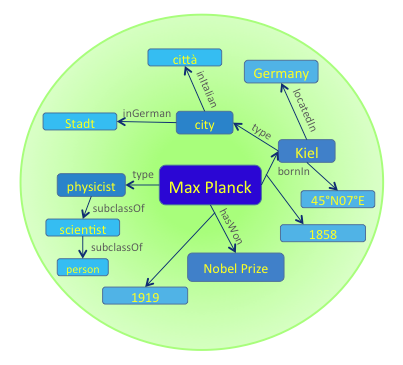
\includegraphics[width=11cm]{yago.png}
\caption{YAGO}

\end{figure}
\subsection*{Différentes approches d'annotation temporelle}			
\subsubsection{Introduction}
\paragraph{}
Dans le domaine du Web sémantique, il y a plusieurs extensions de RDF qui ont été proposé pour : la vérité, la confiance, la certitude, le temps ect…
Par exemple : Pour la verité de certaines triplets où le degré de la vérité est entre $0$ et $1$, l’instance “Rome is a big city to degree 0.8” peut être représentée par $(Rome, type,big{\_}city) : 0.8$.
\subparagraph{}
De même pour la certitude un autre forme a été proposé :
$(Max,hasSupervisor : (0.9,2003),William)$ à la forme générale suivante $(s, p : (x,t),o)$
\newline
La certitude $x$ est représentée sous forme d'un pourcentage, 90\% pour cet exemple.
\subsubsection*{L'annotation temporelle}
\paragraph{}
La nécessité de l’annotation temporelle sur les documents Web a été évoqué dans des nombreux travaux de recherche. La première approche formelle au problème de modélisation et d’interrogation temporelle en RDF a été introduite par Gutierrez et al~\cite{gutierrez2005}.
\subparagraph{}
Ensuite, Udrea et al~\cite{udrea2006} ont remis en question la notion d'annoter temporellement les graphes RDF et depuis plusieurs travaux de recherche ont évoqué cette problèmatique.
Ces derniers définissent le triplet annoté de la forme suivante $(s,p:t,o)$, $t$ est une étiquette temporelle.
De plus ils ont donné des algorithmes pour interroger les données RDF annotées.	

\subsection*{RDF Temporel ou tRDF}
\paragraph{}
Pour introduire RDF temporel ''tRDF'' on commence par les exemples suivants:
\newline
Il y a des triplets comme par exemple : " Mary est toujours la mère de John " qui n'ont pas une caractéristique temporelle explicite parce qu'il est toujours valide. Mais il y a aussi des triplets ayant une valeur vrai que dans une plage temporelle bien précise, par exemple : " Bill Clinton est le président de Etats Unis ", n'est valide que dans l'intervalle $[1993-2001]$.
\subparagraph{}
Donc il y a des triplets qui ne peuvent être reconnus que dans des périodes temporelles précises.
\paragraph{}
D'après Andrea et al~\cite{pugliese2008} l’annotation tRDF peut être exprimé de la manière suivante ($n$ est un nombre entier, $T$ appartient à un interval de temps, $s$ le sujet, $p$ le prédicat, $v$ l'objet) :
\begin{enumerate}
\item ($s$, $p$ : {$T$}, $v$), ce type de triplet représente une relation entre le sujet et le prédicat et l'objet dure un temps $T$ (dans n'importe quel point de temps dans $T$).
\item $($s$, $p$ : <$n$ : $T$>, $v$)$, ce triplet présente une relation entre $s$, $p$ et $v$ qui dure au moins n point de temps différents dans $T$.
\item ($s$, $p$ : [$n$ : $T$], $v$), ce triplet présente une relation entre $s$, $p$ et $v$ qui dure au plus $n$ points de temps différents dans $T$.
\end{enumerate}
\subsection*{L'importance de l'annotation temporelle dans LOD}
\subsubsection*{Présentation du LOD}
\paragraph{}
\gls{lod}\footnote{http://linkeddata.org/}, c'est un moyen de publier des données structurées sur le Web où les données contenues dans des bases de données sont exposées sur le Web avec leur sémantique, ce qui donne la possibilité au métadonnées d'être connectées et enrichies d'une manière solide, permet d'avoir plusieurs représentations d'un même contenu et fait des rapprochements entre des ressources connexes.
\subparagraph{}
Au cours des dernières années, le Web de donnée a développé dans une grande fusion de divers ensemble de données provenant de plusieurs domaines. Ce dernier décrit les ressources identifiées par des \gls{uri} en représentant leurs propriétés et des liens vers d’autres ressources. L'ensemble des données fournit des connaissances du monde réel.
\subsubsection*{Relation entre l'annotation temporelle et LOD}
\paragraph{}
Les informations sur un intervalle temporel de validité pour les évènements décrits par des triplets RDF jouent un rôle important dans un grand nombre d'applications.
Un grand nombre de triplets dans LOD ne sont valides que dans un certain intervalle de temps qu'ils l'appellent la protée de leurs temps.
Par exemple dans DBpedia ils indiquent que "Mario Balotelli joue pour les équipes AC Lumezzane et le Milan AC". Lorsqu'on modélise des connaissances du monde réel, Mario Balotelli ne peut pas jouer au même temps avec AC Lumezzane et le Milan AC.
\subparagraph{}
Les logiques temporelles d'informations ont besoin d'avoir de la protée temporelle des faits tels que “Mario Balotelli joue pour l'équipe AC Milan”.
Une approche a été proposée pour détecter la portée des évènements visés par des triplets RDF par Rule et al~\cite{rula2013}, elle se compose de quatre étapes principales~:
\begin{itemize}
\item Les données du document Web sont normalisées pour tenir compte de l’importance des dates figurants dans les documents.
\item La sortie de la phrase est comparée avec un ensemble d’intervalles de temps pertinents pour obtenir des notes de significations pour chaque intervalle.
\item Un ensemble d’intervalles plus importants est sélectionné.
\item Les intervalles sélectionnés sont fusionnés lorsque c’est possible.
\end{itemize}
\subparagraph{}
La plateforme DeFacto(Deep Fact Validation)~\cite{lehmann2012} a été utilisée pour la validation des états on cherchant des sources qu'elle confirme sur le Web.
\subparagraph{}
Les triplets sont représentés par des faits et peuvent être associé à un contexte temporelle.
Par exemple, $<Balotelli, team, AC Milan>$ se réfère à un événement de $2003-2009$, une annotation temporelle est rattachée au fait comme suit $<f, [ti,tj]>$.
\subparagraph{}
Cette approche combine deux types d'informations~: les informations temporelles recueillies dans des documents Web et les informations temporelles contenues dans les bases de connaissances, pour associer des intervalles de temps au triplets RDF.
\subsection*{Temps valide des triplets dans les données géospatiales liées}
\paragraph{}
Bereta et al~\cite{bereta2013} introduisent la composante temporelle des données du modèle stRDF et le langage de requêtes stSPARQL, récemment proposés pour la présentation et l’interrogation des données géospatiales liées qui changement dans le temps.
\subparagraph{}
L’introduction du temps dans les modèles de données et les langages de requêtes, a été l’objet de recherches approfondies dans le champs des bases de données relationnelles.
\subparagraph{}
Les trois types distincts de temps qui ont été étudiées~:
\begin{itemize}
\item L'action temporelle indépendante, par exemple ($01/12/1954$ c’est l’anniversaire de John).
\item Le temps d’évènement ou un fait vrai dans l’application (entre $2001-2012$ John a été professeur).
\item Le délail de transaction qui est le moment où un fait est en cours dans la base de données (l’heure système qui présente l’heure exact quand John est un professeur "$2001-2012$" est en cours dans la base de données).
\end{itemize}
\paragraph{}
Bereta et al~\cite{bereta2013} présentent également le concept de horodatages anonymes dans les graphes RDF, par exemple le quadruplet(quad) de la forme $(s, p, o)[t]$, où $t$ est une horloge ou un timestamp $x$ anonyme déclarant que le triplet est valable dans un certain point de temps inconnue.
\subparagraph{}
L’idée principale est d’intégrer les informations géospatiales pour le modèle de graphe RDF temporel. Le langage d’interrogation \gls{stsparql}\footnote{http://www.strabon.di.uoa.gr/stSPARQL}, ajoute deux nouveaux types de variables spatiales et temporelles, aux variables SPARQL standards.
\subsection*{Base de données temporelles}
\paragraph{}
Une base de données temporelle est une base de données avec des acpects de temps intégrés(temps-valide, temps-transaction), c'est à dire un modèle de données temporelles et une version temporelle du langage structuré de requête(SPARQL, SQL).
\subparagraph{}
En effet, le \textit{temps valide} dénote la période du temps durant laquelle un fait est vrai par rapport à la réalité.
Le \textit{temps-transaction} est la période de temps pendant laquelle un fait est stocké dans une base de données.
\paragraph{}
Dans le contexte de l'annotation temporelle des graphes RDF, les besoins se résume comme suit~:
\begin{itemize}
\item L'accès à des différents versions d’une ontologie.
\item Récupération des informations passées sur les sites Web.
\item La distribution des mise à jour des journaux.
\end{itemize}
\subparagraph{}
En vertu des travaux de Antoniou et al~\cite{antoniou2004} présentent une ontologie du service Web, pour monter qu'une ontologie peut passer par plusieurs états, ainsi que d'autres recherches dont l'objectif d'analyser et justifier les besoins cités auparavant.
\paragraph{}
Une base de données temporelle peut être exprimé comme un répertoire d'informations temporelles.
Gutiérrez et al~\cite{gutierrez2007}, montrent qu'il y aura deux manières pour ajouter des dimensions temporelles dans un graphe RDF intemporel~:
\begin{itemize}
\item Étiqueter les éléments soumis à des changements, les triplets par exemple, à chaque changement un nouveau graphe créer et l’ancien état sera stocké quelque part.
\item Versionner : capture de temps de transaction, l’étiquetage est mieux que les versions pour les raisons suivantes:
\begin{itemize}
\item Il conserve le principe de la nature distribuée et extensible de RDF.
\item Si la nouvelle version n’affecte que quelques éléments cela implique la création d’un nouveau graphe, de ce fait on aura des contraites de mémoire.
\end{itemize}
\end{itemize}
\paragraph{}
Gutiérrez et al~\cite{gutierrez2007}, ont travaillé sur le domaine temporel à base de points et ils ont aussi codé les points du temps en intervalle.
\subparagraph{}
Ces derniers ont proposé un vocabulaire pour affirmer les moments où les triplets sont valables dans un graphe RDF.
\subsection*{Graphe Temporel}
\paragraph{}
Un graphe temporel c'est des triplets$(s,p,o)$ avec des étiquettes temporelles qui représentent la période dans laquelle il est valable dans le monde réel.
Exemple le triplet $(s,p,o)$ est valable dans un temps $t$, $(a,b,c)[t]$, ou autrement dans un intervalle de temps $[t1,t2]$, $(a,b,c)[t1,t2]$.
\subparagraph{}
L'idée générale de Pugliese et al~\cite{pugliese2008} est d'annoter RDF avec un interval de temps.
Ces derniers ont proposé un graphe temporel d'indexation "tGRIN". C'est une structure d’indexation qui construit un index spécialisé pour RDF temporels qui sont stockés dans une base de données relationnelle "RDBMS".
\subparagraph{}
D’autres efforts pour stocker RDF dans une base relationnelles:
\begin{itemize}
\item Jena2 de Apache
\item Sesame de openRDF.org
\item 3store ou triplestore de University of Southampton
\end{itemize}
\paragraph{}
D'autes index temporels sont implémentés ( R+ trees, SR-trees, ST-index, and MAP21) mais l'index tGRIN présentent des performances supérieures selon les expérimentations faites dans~\cite{pugliese2008}.
\subsection*{Synthèse}
\paragraph{}
Plusieurs travaux de recherches on été mis au point pour résoudre le problème des données qui présentent un sémantique temporel dans les graphes RDF. Nous avons étudié ces travaux afin d'avoir une vision globale sur la problèmatique et pour voir ce qui est déjà fait dans ce domaine. On s'inspire de ces travaux pour proposer une nouvelle approche qui soit satisfaisante pour annoter temporellement les métadonnées de Wikipedia.
\subsection*{Extraction des données}
\subsubsection*{Introduction}
\paragraph{}
L'extraction, la fouille de données, ou encore la fouille des connaissances à partir de données, ont pour objet l'extraction d'un savoir, d'une connaissaince, ou dans notre cas une connaissance mise en relation temporelle à partir de grandes quantité de données par des méthodes automatiques.
\subsubsection*{Différentes approches de l'extraction }
\paragraph{}
Une approche proposée par Zweigenbaum et Tannier~\cite{zweigenbaum2013} consiste à détecter les relations temporelles entre les évènements et les expressions temporelles à partir des comptes rendu hospitaliers.
\subparagraph{}
La détection des relations temporelles entre les évènements dans un texte, fournit de bonnes informations pour l’extraction.
\newline
C’était les défis de TempEval Verhagen et al~\cite{verhagen2010} qui ont abordé en “domaine ouvert”, en cherchant à détecter en TempEval2 cinq types de relations temporelles :
\newline
$(Before, After, Overlap, Before\_or\_Overlap, Overlap\_or\_Before)$
et Identifier les relations temporelle décrivant la chronologie du séjour hospitalier.
\newline
Les relation à trouver dans des différentes situations :
\begin{itemize}
\item{}Entre un événement et une date ou autre événement qui domine.
\item{}Entre un événement et la date de création de cette élément.
\item{}Entre deux événement principaux de deux phrases consécutives.
\end{itemize}
Identifier les informations temporelles décrivant la chronologie entre ces événements.
\subparagraph{}
Ces derniers utilisent des différents classifieurs (table de décision, arbre de décision, JRip, classifieurs bayésien naif) et le classifieur à arbre de décision J48 implémenté dans weka.
\subparagraph{}
La question c’est d’identifier les situations les plus importantes à traiter et les méthodes à utiliser.
Zweigenbaum et Tannier~\cite{zweigenbaum2013} utilisent une méthode d’apprentissage supervisé avec un ensemble de données et des classifieurs entrainés pour chaque situation.
L'évaluation a été appliquée sur un corpus d’apprentissage qui contient 190 échantillons, dont 120 échantillons de test.
\subparagraph{}
On peut utiliser cette méthode pour les propriétés de DBpedia à la place des ces comptes rendus hospitaliers et chercher à chaque fois d'apprendre à partir d'un motif qui peut être temporel, spacial, ect...
Au lieu d’une procédure de décision gloutonne ou aléatoire, une relation de décision globale pourrait être implémentée pour étudier toutes les relations temporelles prédites.
\paragraph{}
Le but de Kessler et al~\cite{kessler2013} est d'extraire les dates saillantes (importantes) qui méritent de figurer dans une chronologie événementielle.
Ces derniers ont utilisé une approche d’apprentissage pour extraire les dates saillantes pour un thème donné.
\subparagraph{}
La méthode consiste d'annoter automatiquement les informations événementielles. C’est à dire repérer et baliser (Event) les occurrences d’événements au sens TimeML\footnote{http://timeml.org/site/index.html} et de les classifier selon l’ontologie définie par le schéma d’annotation.
\subsubsection*{Synthèse}
\paragraph{}
L'extraction des informations temporelles est une étape primordial. On pourrait s'inspirer des méthodes présentées précédemment pour répondre aux objectifs fixés au démarrage de cette étude.
\bibliographystyle{alpha}
\bibliography{Biblio.bib,w3c.bib}
\printglossary[title=Glossaire]
%\glsaddall
\end{document}

